%%%%%%%% ICML 2021 EXAMPLE LATEX SUBMISSION FILE %%%%%%%%%%%%%%%%%
\documentclass{article}
\usepackage[]{algorithm2e}
\usepackage{algorithmic}
\usepackage{algorithm}
% Recommended, but optional, packages for hs and better typesetting:
\usepackage{microtype}
\usepackage{graphicx}
\usepackage{amsmath}
\usepackage{appendix}
\usepackage{subfigure}
\usepackage{booktabs} % for professional tables
\usepackage{hyperref}
% Attempt to make hyperref and algorithmic work together better:
\newcommand{\theHalgorithm}{\arabic{algorithm}}
\usepackage{icml2021}
\usepackage{float}
\usepackage{enumitem}

\begin{document}
\twocolumn[
\icmltitle{Reinforcement Learning 2024
Assignment 3: Policy-based Reinforcement Learning}

\icmlsetsymbol{equal}{*}
\begin{icmlauthorlist}
\icmlauthor{Sherry Usman}{equal,to}
\icmlauthor{Qin Zhipei}{equal,to}
\icmlauthor{Megan Mirnalini Sundaram R}{equal, to}
\end{icmlauthorlist}

\icmlaffiliation{to}{Leiden University}

% You may provide any keywords that you
% find helpful for describing your paper; these are used to populate
% the "keywords" metadata in the PDF but will not be shown in the document
\icmlkeywords{Machine Learning, Deep Q-Learning, Experience Replay, Target Network}

\vskip 0.3in
]

\begin{abstract}

\end{abstract}

\section {Introduction}
In this paper we will delve into the Lunar Lander environment taken from the OpenAI Gym library. The Lunar Lander game is a classical reinforcement learning environment where the goal is to optimise the trajectory of our rocket such that it lands between the two flags. 

\begin{figure}[htbp]
\centering
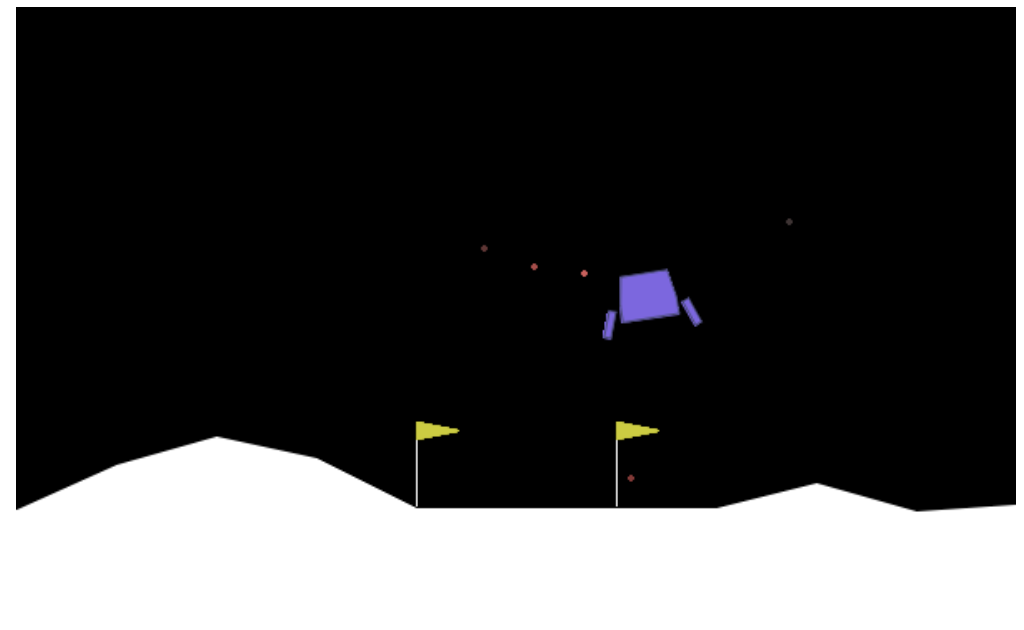
\includegraphics[width=0.6\linewidth]{Report/images/visualisation.png}
\caption{\label{fig:Visualization of the Cart-pole} A visualisation of the Lunar Lander problem}
\end{figure}



The action space and the observation space of our environment is shown below. 


\begin{table}[htbp]
\centering
\begin{tabular}{|l|c|}
\hline
\textbf{Value} & \textbf{Action} \\
\hline
0  & Do nothing \\
\hline
1 & fire left orientation engine \\
\hline
2  & fire main engine \\
\hline
3 & fire right orientation engine  \\
\hline
\end{tabular}
\caption{Action Space}
\label{tab:hyper-parameters}
\end{table}

The observation space is an 8-dimensional vector, the positional coordinates of the lunar lander (x and y), its linear velocities in x and in y respectively, its angle, its angular velocities and two boolean values that represent whether each leg is in contact with the ground or not. 

\section{Algorithm Variation}
Policy based reinforcement learning is mostly used for continuous action spaces. In policy-based reinforcement learning, there is no value function which determines the next best possible action. Instead, it uses a parameterized policy. A value function may be used for learning the best policy, but not for selecting the action. The implemented policy is then improved, based on the data from each episode using policy gradient methods. \cite{sutton-barlo}
The outline of policy-based algorithms is using a parameterized policy function, which is denoted by $\pi_\Theta$. 
Here, $\theta$ refers to the parameters of the function and $\pi$ refers to the function itself. After defining the policy function, a path $\tau$ is chosen. If $\tau$ is good, then the parameters $\theta$ are increased towards the path $\tau$. Otherwise, it is decreased. In this way, it is maintained until the goal is reached.    \cite{plaat-deeprl}
The various algorithms that were implemented to realise this approach are
\subsection{REINFORCE}
\quad REINFORCE is a commonly used Monte-Carlo Policy Gradient algorithm. As mentioned above, the parameters of the policy is defined by $\theta$. Therefore, the quality of such parameters for the state to action probabilities for the policy is given by $J(\theta)$. To improve the gradient, the differential of the parameters are taken. 

\newline The quality is given by $\mathbb{E}_\pi [ \sum _a q_\pi(S_t, a)\nabla_\pi(a|S_t, \theta)]$

\newline The update of these functions happen in a Monte-Carlo function i.e., random sample. The function is updated after an entire trajectory/path is completed. Therefore, this happens in an off-policy way.  

\subsection{Actor - Critic}
Unlike REINFORCE, Actor-critic Methods consists of two functions - the actor and the critic. The actor refers to the policy function and the critic refers to the value functions. Similar to an actor and a critic, the actor (policy) function focuses on the path to be taken, and the critic evaluates the said path, by computing the value function. 
The focus on the algorithms is based on policy gradients. \cite{actor-critic}
\newline As used in REINFORCE, the policy gradient is given by 
\newline 
$\nabla_\theta J(\theta) = \mathbb{E}_\pi[\sum _{t=0}^{T-1} \nabla_\theta log\pi_\theta (a_t|s_t)G_t]$
\subsubsection{Bootstrapping}
The main difference from REINFORCE, is that actor-critic algorithms employ bootstrapping to counteract the low bias and high variance (since the action selection in REINFORCE is random). The actor-critic is a combination of the best of both policy-based and value-based methods. It combines the advantage of having a low variance from the value method, and the advantage of having a high bias from the policy method.
However, there might be high variance in the rewards and gradient estimate. To counteract this, bootstrapping is used. 

\subsubsection{Baseline Subtraction}
\subsubsection{Bootstrapping and Baseline Subtraction}

\section{Goals Achieved}
\subsection{Effects of policy gradients on variance}
\subsection{Effects of bootstrapping on the policy gradients}
\subsection{Comparison of Performance}
\subsection{Effect of entropy regularization on performance}

\bibliography{Report/references}
\bibliographystyle{Report/reference_style}
\end{document}

